\noindent

\includegraphics[height=1.25cm]{images/pictograms/replication}

\includegraphics[height=1.25cm]{images/pictograms/benchmark}

\includegraphics[height=1.25cm]{images/pictograms/FEM}

\includegraphics[height=1.25cm]{images/pictograms/paraview}

%%%%%%%%%%%%%%%%%%%%%%%%%%%%%%%%%%%%%%%%%%%%%%%%%%%%%%%%%%%%%%%%%%%%%%%%%%%%%%%%%%%%%%%%%%%%%%%%%%%

\begin{flushright} {\tiny {\color{gray} python\_codes/fieldstone\_25/text.tex}} \end{flushright}

\par\noindent\rule{\textwidth}{0.4pt}

\begin{center}
\inpython
{\small Code: \url{https://github.com/cedrict/fieldstone/tree/master/python_codes/fieldstone_25}}
\end{center}

\par\noindent\rule{\textwidth}{0.4pt}

Last revision: March 11th, 2025.

\par\noindent\rule{\textwidth}{0.4pt}

%%%%%%%%%%%%%%%%%%%%%%%%%%%%%%%%%%%%%%%%%%%%%%%%%%%%%%%%%%%%%%%%%%%%%%%%%%%%%%%%%%%%%%%%%%%%%%%%%%%

This numerical experiment was first presented in \textcite{vaks97} (1997).
It is detailed in Section~\ref{MMM-ss:vaks97}.
It consists of an isothermal Rayleigh-Taylor instability in a two-dimensional box
of size $L_x=0.9142$ and $L_y=1$.
Two Newtonian fluids are present in the system: the buoyant layer is placed at the bottom of 
the box and the interface between both fluids is given by 
$
y(x)=0.2+0.02\cos \left( \frac{\pi x}{L_x}  \right)
$
The bottom fluid is parametrised by its mass density $\rho_1=1000$ and its viscosity $\eta_1=1,10,100$, 
while the layer above is parametrised by $\rho_2=1010$ and $\eta_2=100$.

No-slip boundary conditions are applied at the bottom and at the top of the box 
while free-slip boundary conditions are applied on the sides. 

In the original benchmark the system is run over 2000 units of dimensionless time and the 
timing and position of various upwellings/downwellings is monitored. 
In this present experiment only the root mean square velocity is measured at $t=0$:
the code is indeed not yet foreseen of any algorithm capable of tracking deformation.
To be clear, this is also not the goal here. We instead want to investigate the 
differences between the $Q_2\times Q_1$ and the $Q_2\times P_{-1}$ (mapped and unmapped)
finite element pairs.

Another approach than the ones presented in the extensive literature which showcases 
results of this benchmark is taken: in this \stone the mesh is initially fitted to the fluids
interface and the resolution is progressively increased. This results in the 
following figure:

\begin{center}
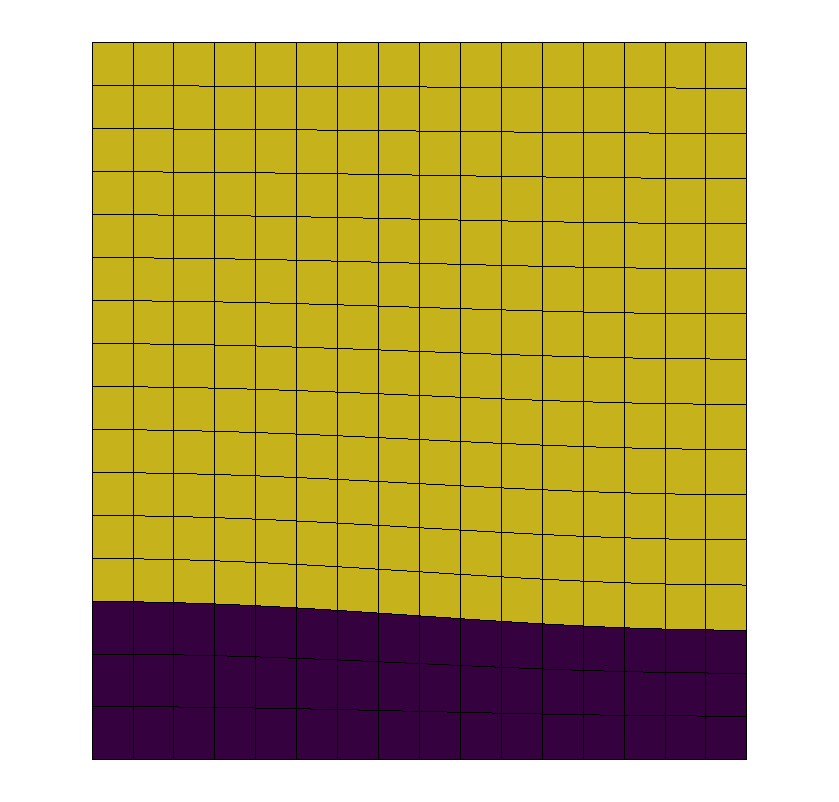
\includegraphics[width=6cm]{python_codes/fieldstone_25/newresults/mats}
\end{center}
Note that in this case each element is assigned a density and a viscosity value that 
is constant over the entire element. 
Note that this approach requires me to compute how many elements are below the interface
for a given resolution. We see on the images below that for meshes $21^2-24^2$ there 
are 4 elements below the interface, for meshes $25^2-29^2$ there are 6 elements, and that 
we get to 7 elements for $30^2$. These steps will be reflected in the measurents presented 
afterwards.

\begin{center}
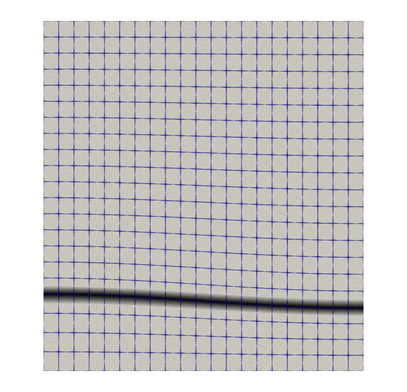
\includegraphics[width=3.42cm]{python_codes/fieldstone_25/images/mesh.0000.jpg}
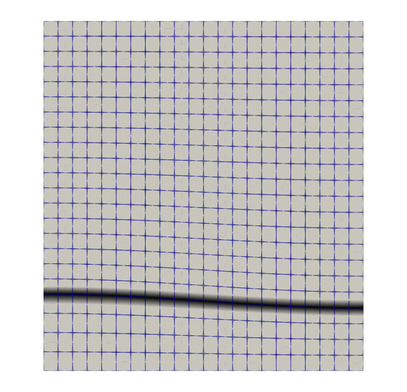
\includegraphics[width=3.42cm]{python_codes/fieldstone_25/images/mesh.0001.jpg}
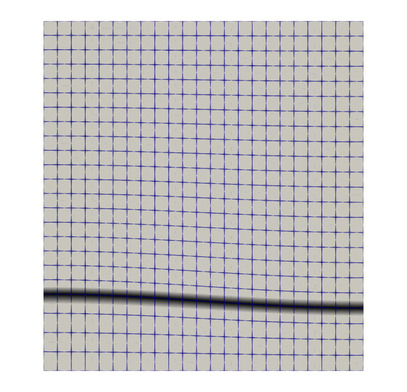
\includegraphics[width=3.42cm]{python_codes/fieldstone_25/images/mesh.0002.jpg}
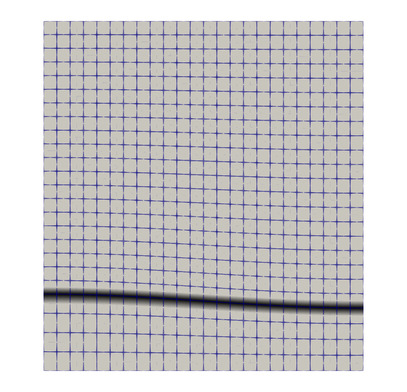
\includegraphics[width=3.42cm]{python_codes/fieldstone_25/images/mesh.0003.jpg}
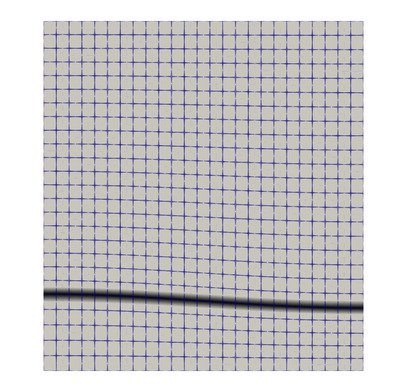
\includegraphics[width=3.42cm]{python_codes/fieldstone_25/images/mesh.0004.jpg}\\
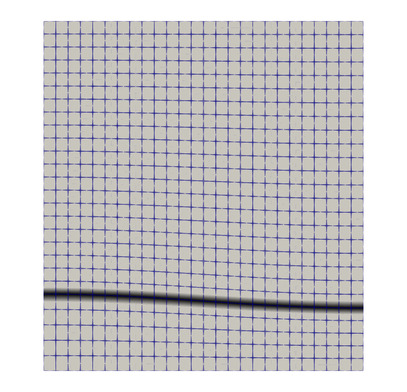
\includegraphics[width=3.42cm]{python_codes/fieldstone_25/images/mesh.0005.jpg}
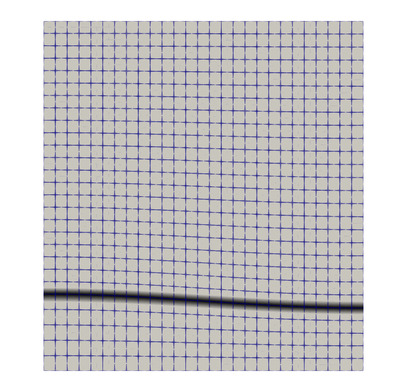
\includegraphics[width=3.42cm]{python_codes/fieldstone_25/images/mesh.0006.jpg}
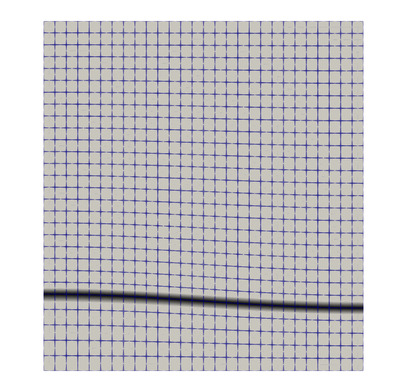
\includegraphics[width=3.42cm]{python_codes/fieldstone_25/images/mesh.0007.jpg}
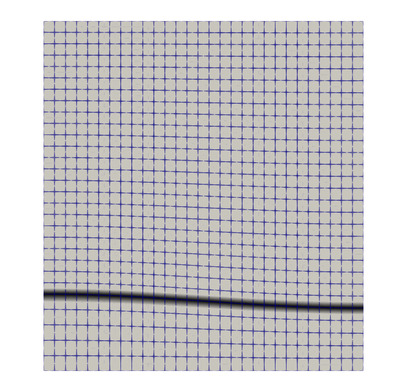
\includegraphics[width=3.42cm]{python_codes/fieldstone_25/images/mesh.0008.jpg}
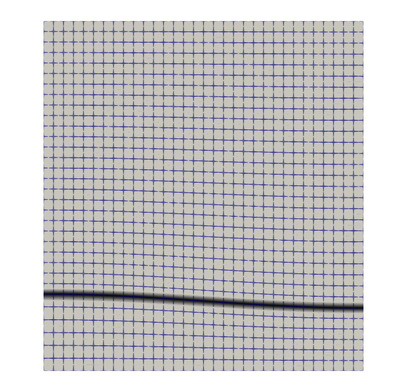
\includegraphics[width=3.42cm]{python_codes/fieldstone_25/images/mesh.0009.jpg}\\
{\captionfont Meshes generated for various resolutions: $21^2$, $22^2$, $23^2$, 
$24^2$, $25^2$, $26^2$, $27^2$, $28^2$, $29^2$ and $30^2$.}
\end{center}

Although it is somewhat a trivial affair to deform the mesh (only the vertical 
position of the nodes is changed), this begs the question as to where the middle node
of the element should be placed for best accuracy?
At this stage I urge the reader to read \stone~76 and come back here afterwards. 

After the mesh has been stretched element edges can be straightened 
(all elements are then trapezes) as parameterized by \lstinline{curved}.  

The code relies on Taylor-Hood elements ($Q_2\times Q_1$), see Section~\ref{MMM-ss:pairq2q1} and 
on $Q_2\times P_{-1}$ elements, see Section~\ref{MMM-ss:pairq2pm1}. 
It has been  benchmarked against the Donea \& Huerta manufactured solution, see Section~\ref{MMM-mms1}.
Isoparametric mapping is used for both element pairs.

Pressure is normalized so that $\int_\Omega p dV= 0$.

Note that there is also a $Q_1\times P_0$ version of the code in the folder.

\newpage
%..............................................................................
\subsection*{Manufactured solution D\&H - $Q_2\times Q_1$ and $Q_2\times P_{-1}$}

\begin{center}
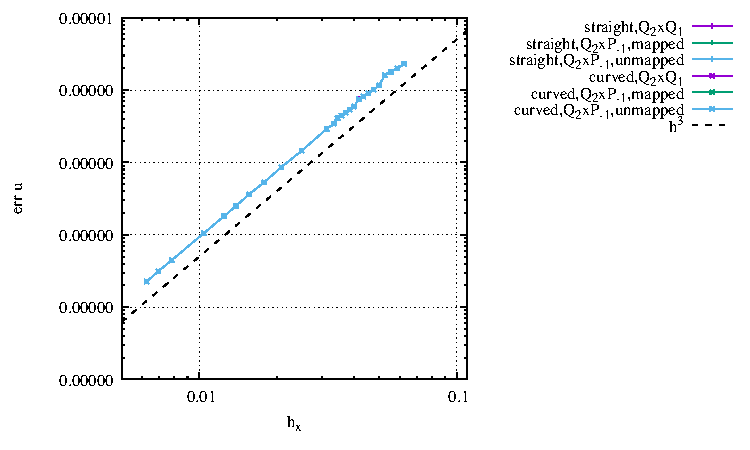
\includegraphics[width=8cm]{python_codes/fieldstone_25/results/doneahuerta/errv.pdf}
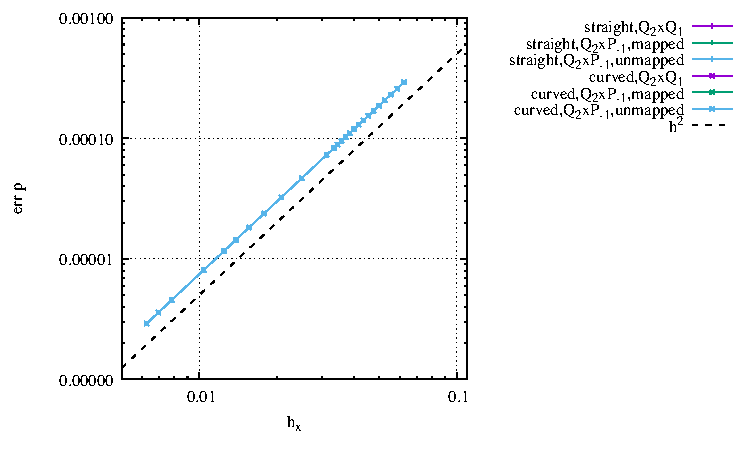
\includegraphics[width=8cm]{python_codes/fieldstone_25/results/doneahuerta/errp.pdf}\\
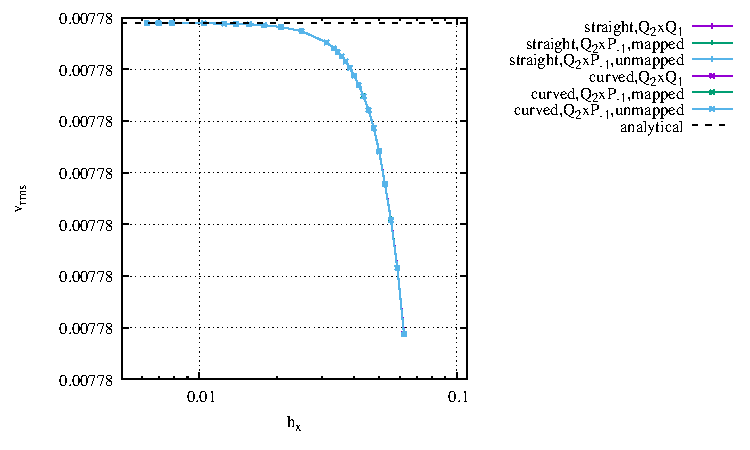
\includegraphics[width=8cm]{python_codes/fieldstone_25/results/doneahuerta/vrms.pdf}
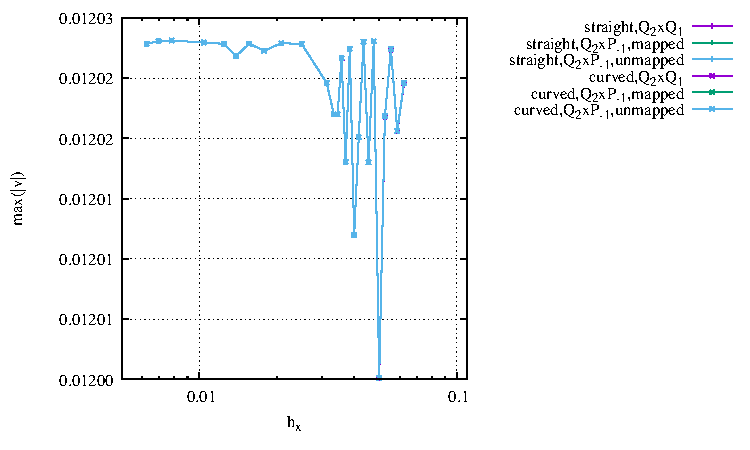
\includegraphics[width=8cm]{python_codes/fieldstone_25/results/doneahuerta/max_vel.pdf}\\
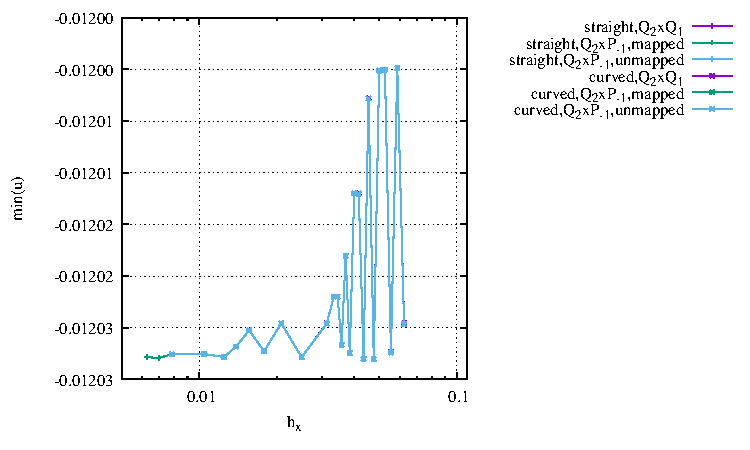
\includegraphics[width=8cm]{python_codes/fieldstone_25/results/doneahuerta/min_u.pdf}
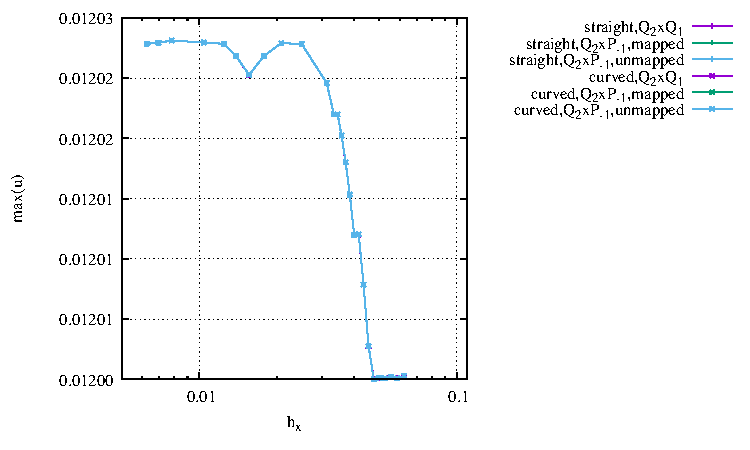
\includegraphics[width=8cm]{python_codes/fieldstone_25/results/doneahuerta/max_u.pdf}\\
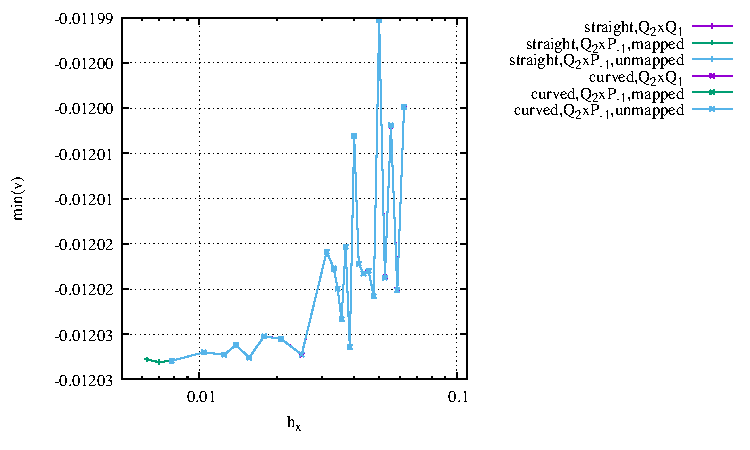
\includegraphics[width=8cm]{python_codes/fieldstone_25/results/doneahuerta/min_v.pdf}
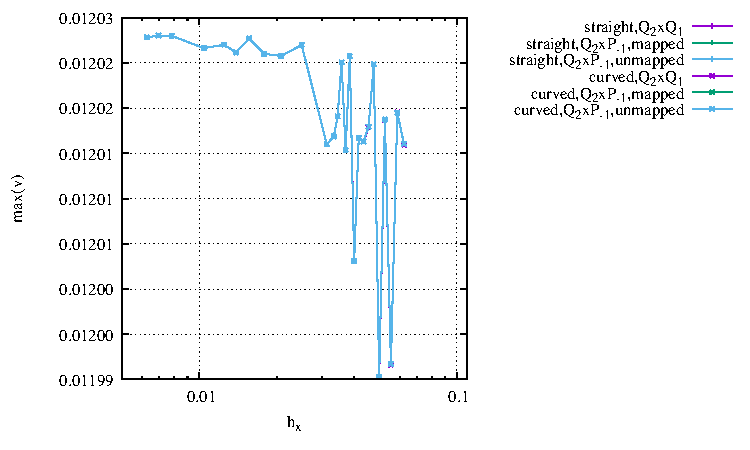
\includegraphics[width=8cm]{python_codes/fieldstone_25/results/doneahuerta/max_v.pdf}\\
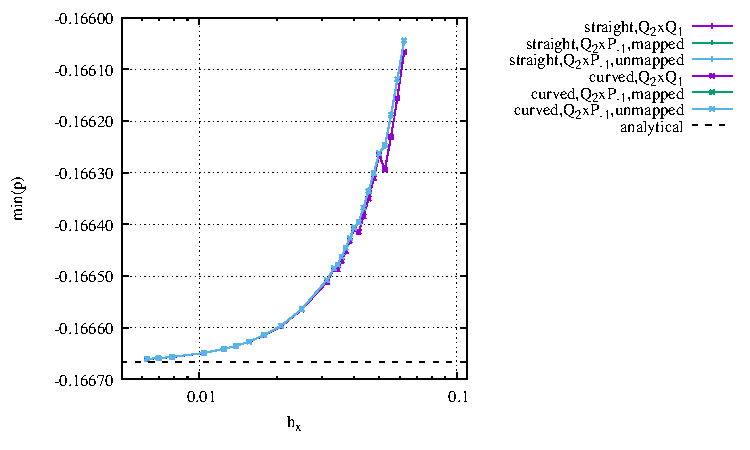
\includegraphics[width=8cm]{python_codes/fieldstone_25/results/doneahuerta/min_p.pdf}
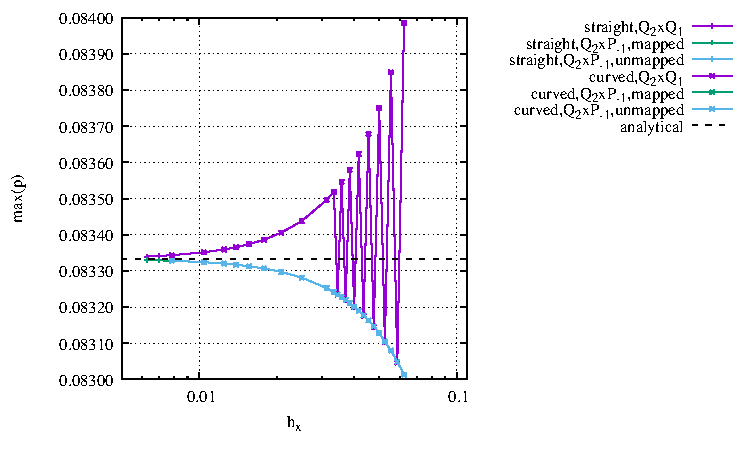
\includegraphics[width=8cm]{python_codes/fieldstone_25/results/doneahuerta/max_p.pdf}\\
\end{center}

\newpage
Velocity measured at the 'interface'
\begin{center}
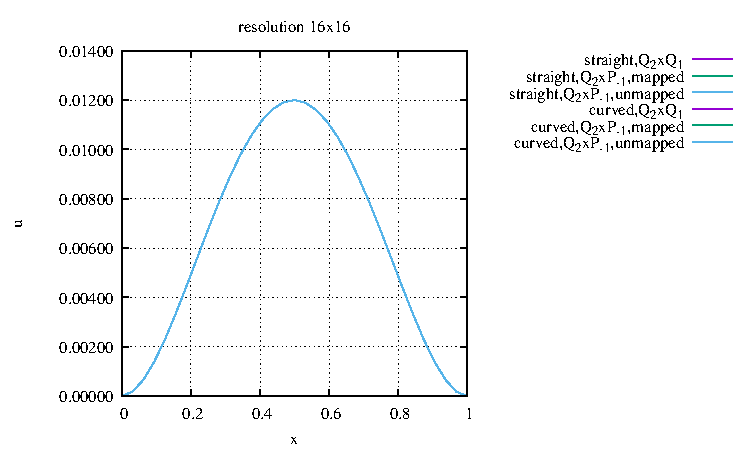
\includegraphics[width=8cm]{python_codes/fieldstone_25/results/doneahuerta/interface_u_16.pdf}
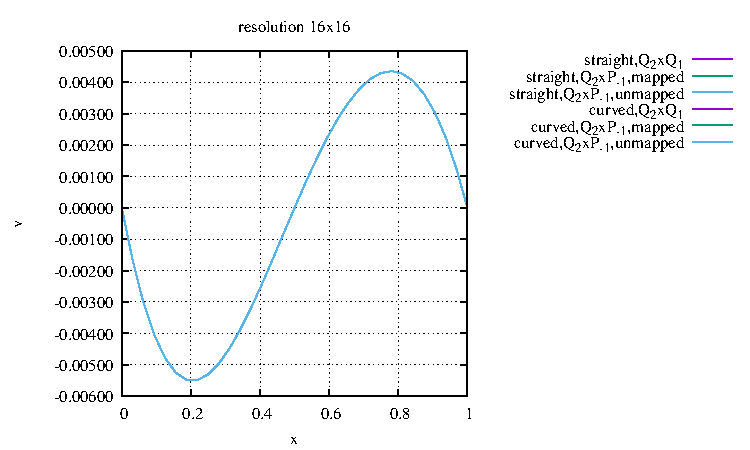
\includegraphics[width=8cm]{python_codes/fieldstone_25/results/doneahuerta/interface_v_16.pdf}\\
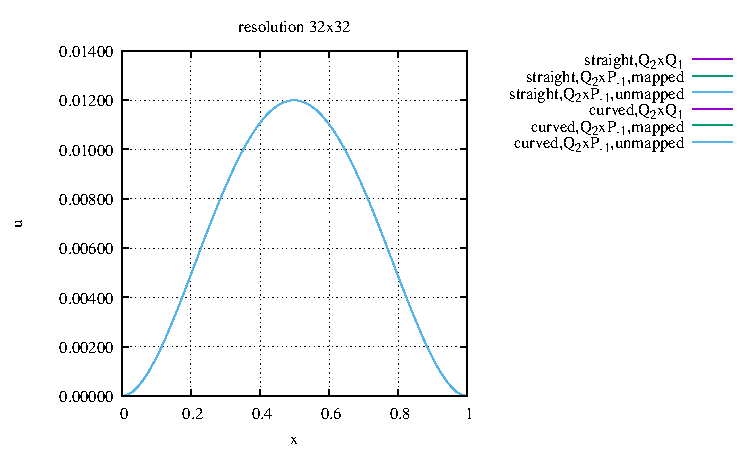
\includegraphics[width=8cm]{python_codes/fieldstone_25/results/doneahuerta/interface_u_32.pdf}
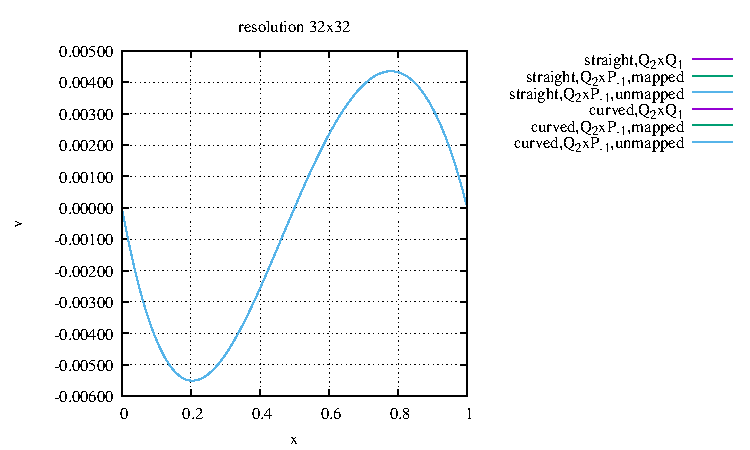
\includegraphics[width=8cm]{python_codes/fieldstone_25/results/doneahuerta/interface_v_32.pdf}\\
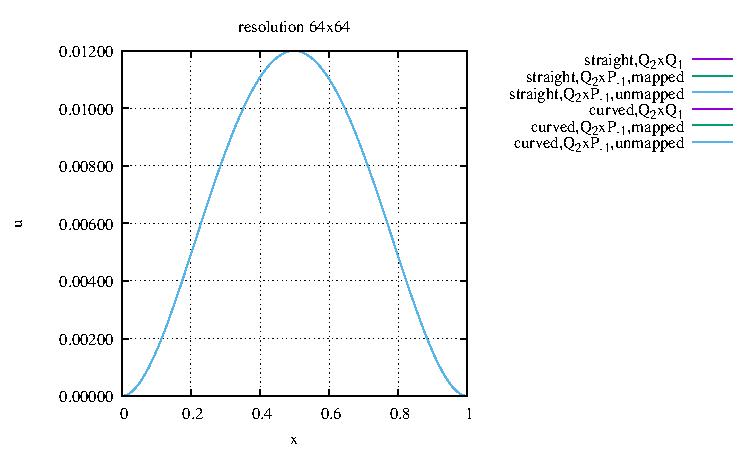
\includegraphics[width=8cm]{python_codes/fieldstone_25/results/doneahuerta/interface_u_64.pdf}
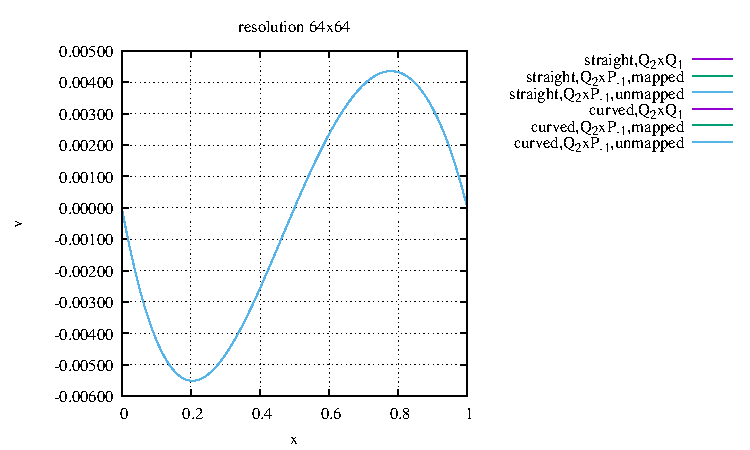
\includegraphics[width=8cm]{python_codes/fieldstone_25/results/doneahuerta/interface_v_64.pdf}\\
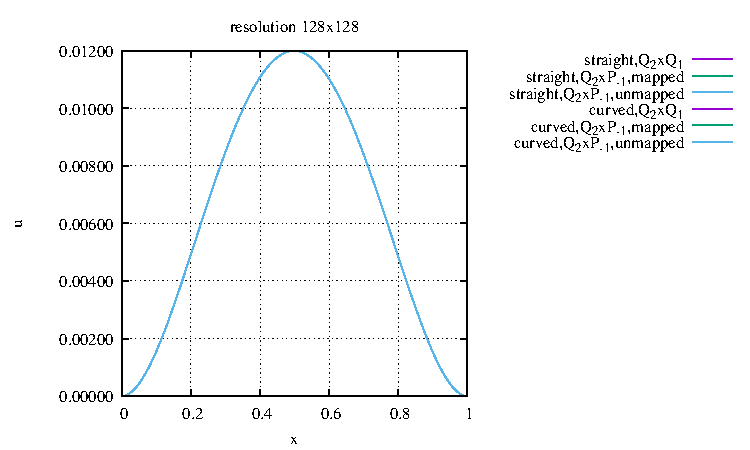
\includegraphics[width=8cm]{python_codes/fieldstone_25/results/doneahuerta/interface_u_128.pdf}
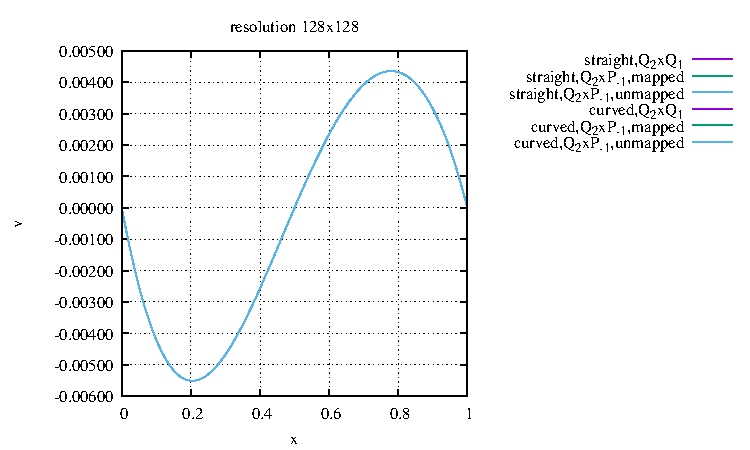
\includegraphics[width=8cm]{python_codes/fieldstone_25/results/doneahuerta/interface_v_128.pdf}\\
\end{center}

\newpage
Pressure measured at the bottom:
\begin{center}
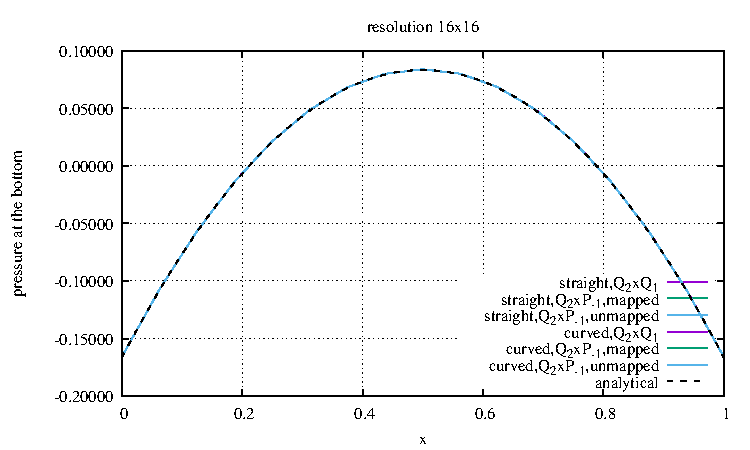
\includegraphics[width=8cm]{python_codes/fieldstone_25/results/doneahuerta/pbottom16.pdf}
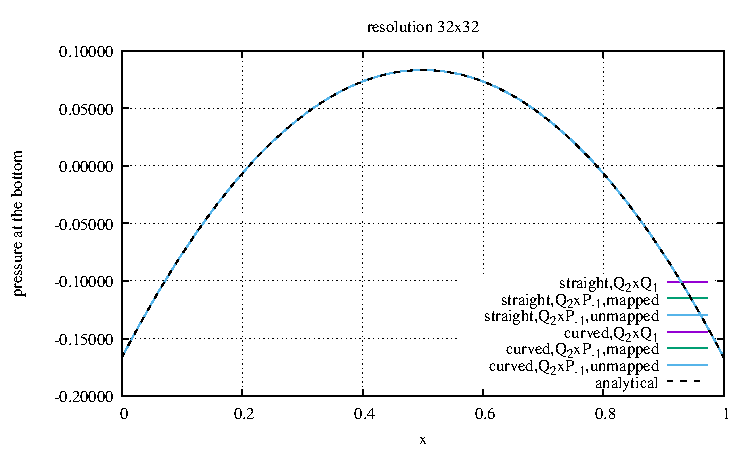
\includegraphics[width=8cm]{python_codes/fieldstone_25/results/doneahuerta/pbottom32.pdf}\\
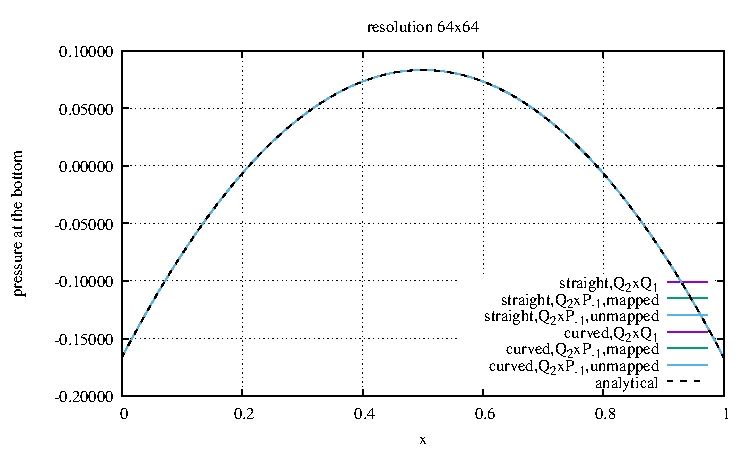
\includegraphics[width=8cm]{python_codes/fieldstone_25/results/doneahuerta/pbottom64.pdf}
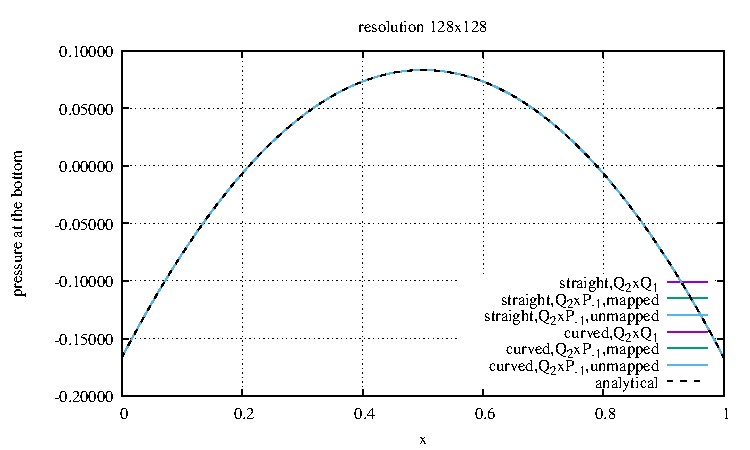
\includegraphics[width=8cm]{python_codes/fieldstone_25/results/doneahuerta/pbottom128.pdf}
\end{center}

The error convergence for velocity and pressure are third and second order 
respectively, as expected. All other measurements are following the analytical solution.

\newpage
%..............................................................................
\subsection*{Isoviscous case - $Q_2\times Q_1$ and $Q_2\times P_{-1}$}

Results are obtained with {\tt script\_errors\_q2} bash script.

\begin{center}
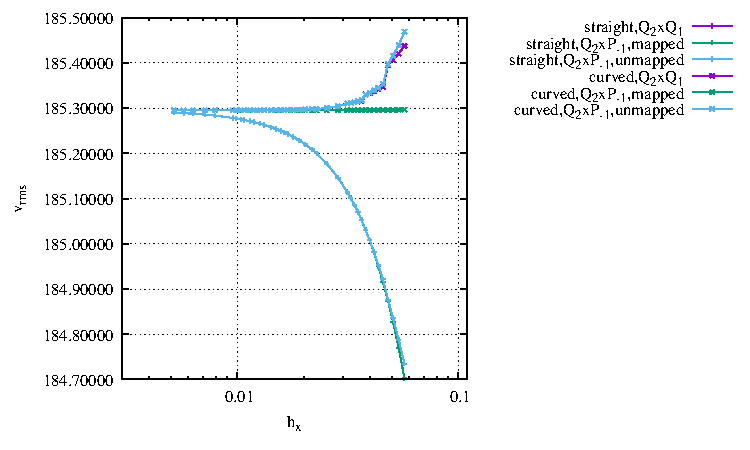
\includegraphics[width=8cm]{python_codes/fieldstone_25/results/isoviscous/vrms.pdf}
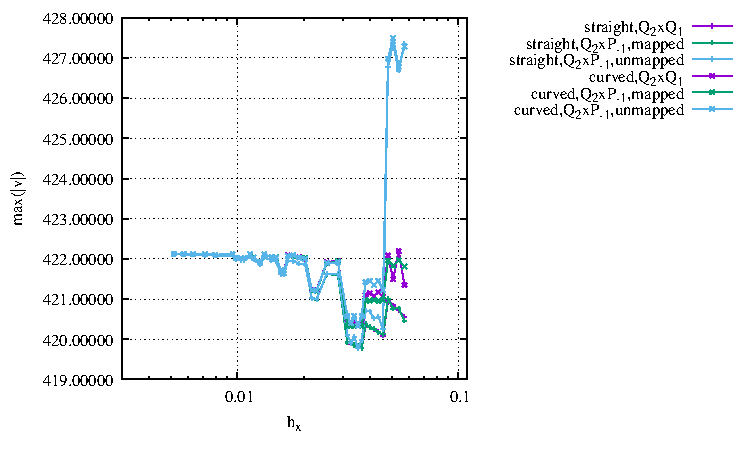
\includegraphics[width=8cm]{python_codes/fieldstone_25/results/isoviscous/max_vel.pdf}\\
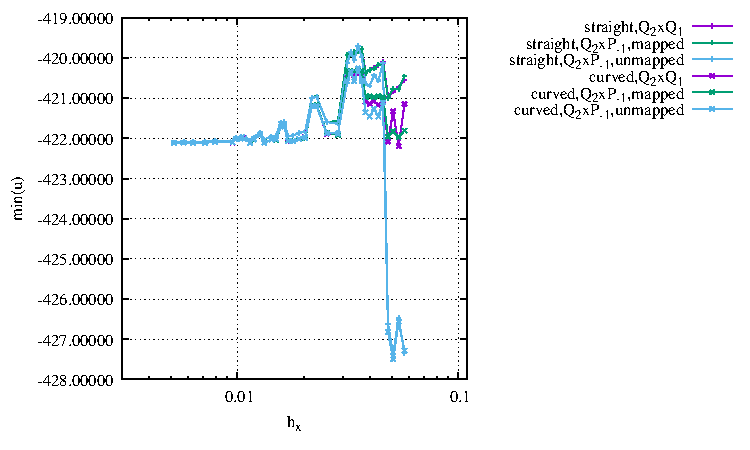
\includegraphics[width=8cm]{python_codes/fieldstone_25/results/isoviscous/min_u.pdf}
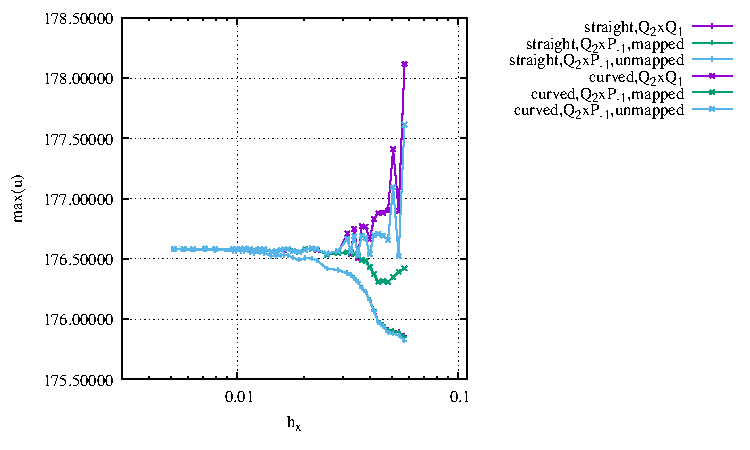
\includegraphics[width=8cm]{python_codes/fieldstone_25/results/isoviscous/max_u.pdf}\\
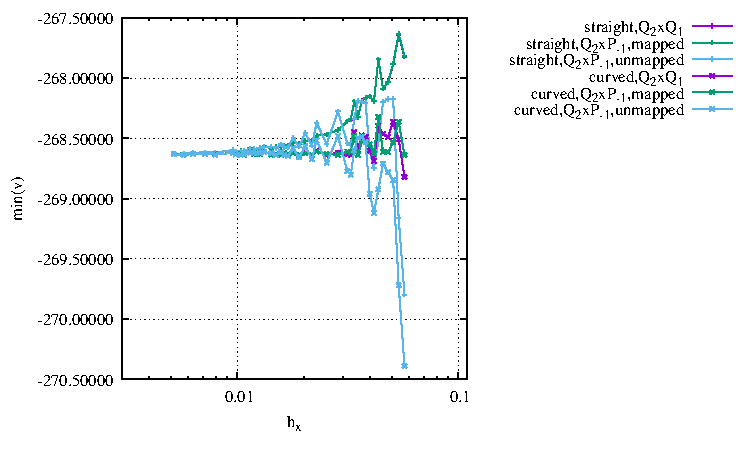
\includegraphics[width=8cm]{python_codes/fieldstone_25/results/isoviscous/min_v.pdf}
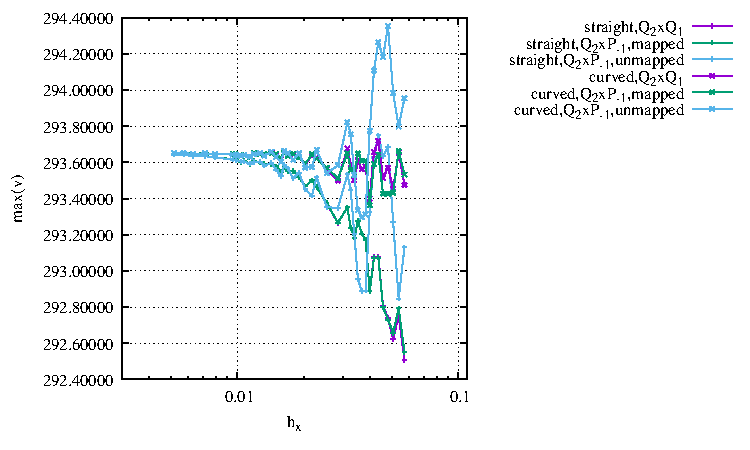
\includegraphics[width=8cm]{python_codes/fieldstone_25/results/isoviscous/max_v.pdf}\\
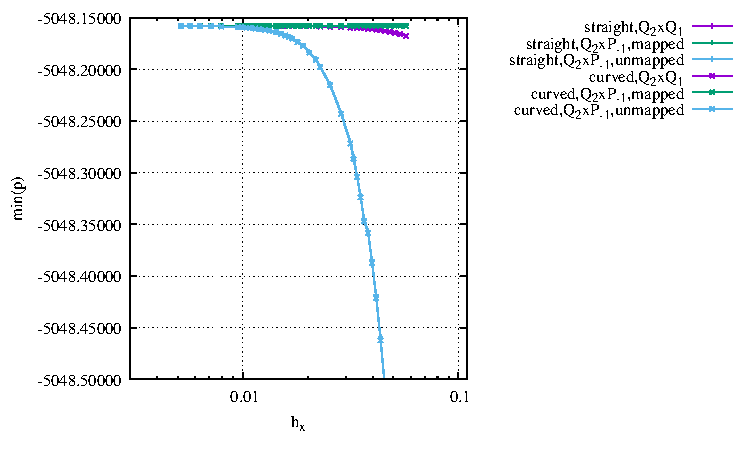
\includegraphics[width=8cm]{python_codes/fieldstone_25/results/isoviscous/min_p.pdf}
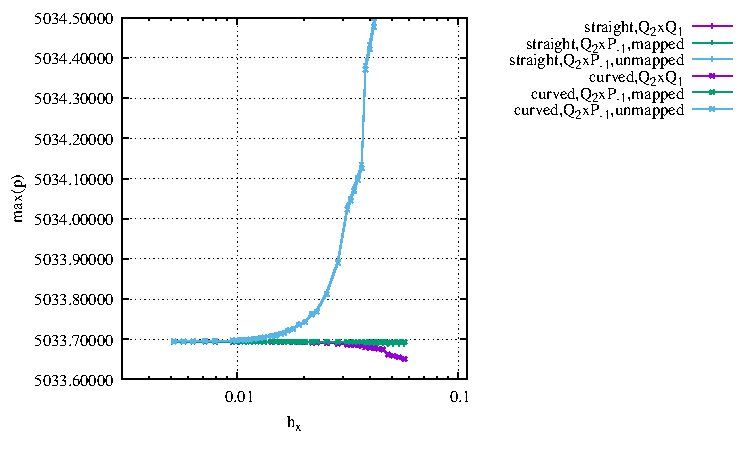
\includegraphics[width=8cm]{python_codes/fieldstone_25/results/isoviscous/max_p.pdf}\\
\end{center}



\newpage
\begin{center}
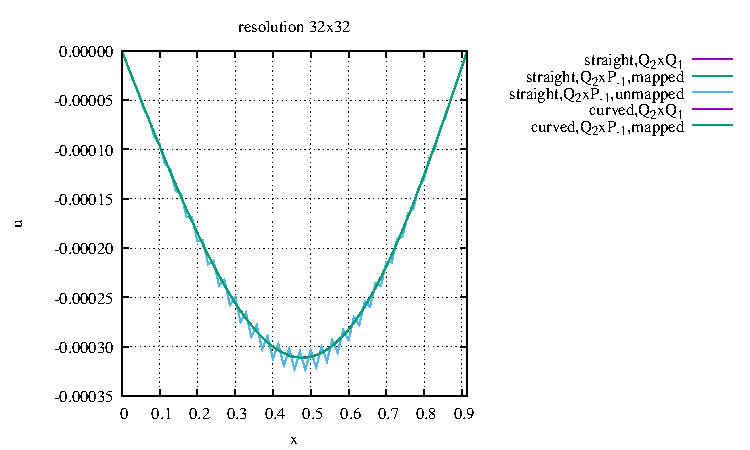
\includegraphics[width=8cm]{python_codes/fieldstone_25/results/isoviscous/interface_u_32.pdf}
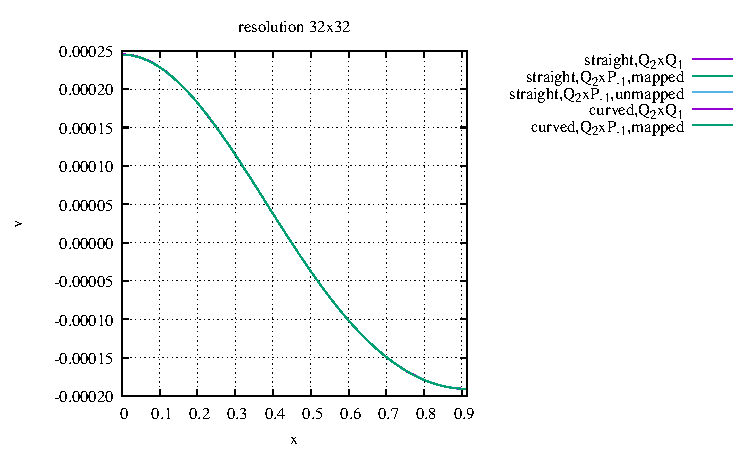
\includegraphics[width=8cm]{python_codes/fieldstone_25/results/isoviscous/interface_v_32.pdf}\\
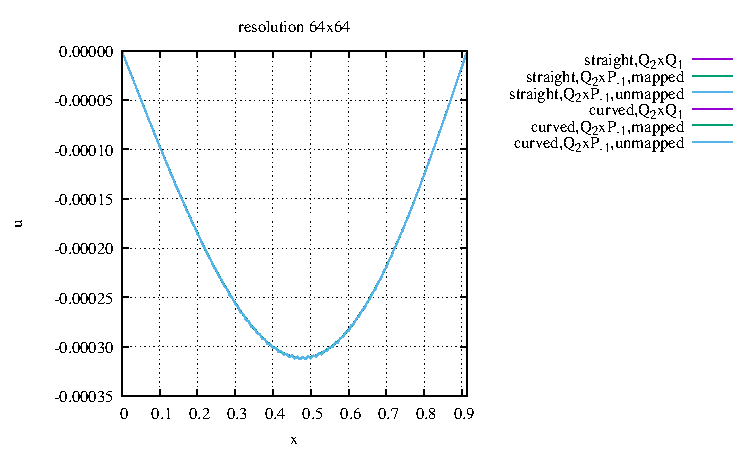
\includegraphics[width=8cm]{python_codes/fieldstone_25/results/isoviscous/interface_u_64.pdf}
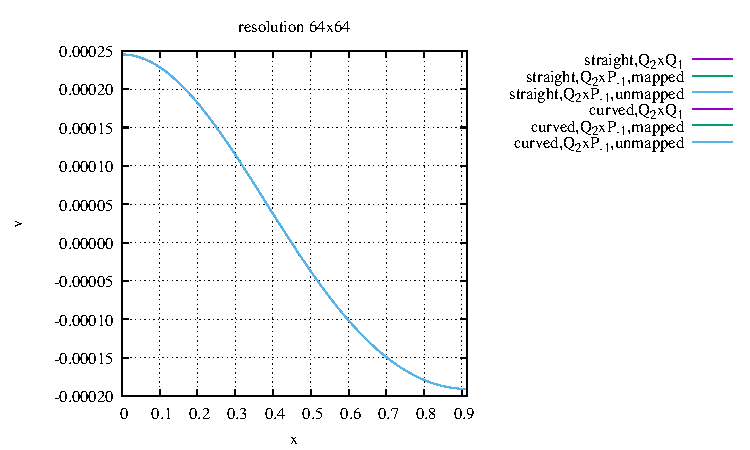
\includegraphics[width=8cm]{python_codes/fieldstone_25/results/isoviscous/interface_v_64.pdf}\\
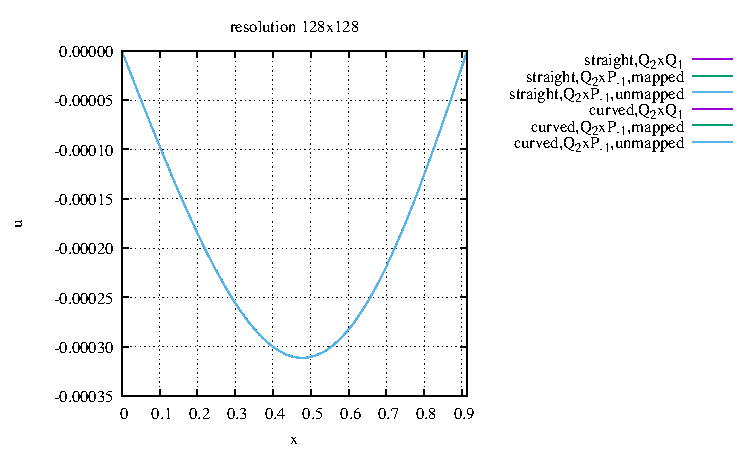
\includegraphics[width=8cm]{python_codes/fieldstone_25/results/isoviscous/interface_u_128.pdf}
\includegraphics[width=8cm]{python_codes/fieldstone_25/results/isoviscous/interface_v_128.pdf}\\
\end{center}

\begin{center}
\includegraphics[width=14cm]{python_codes/fieldstone_25/results/isoviscous/pbottom48.pdf}\\
\includegraphics[width=14cm]{python_codes/fieldstone_25/results/isoviscous/pbottom64.pdf}\\
\includegraphics[width=14cm]{python_codes/fieldstone_25/results/isoviscous/pbottom80.pdf}\\
\includegraphics[width=14cm]{python_codes/fieldstone_25/results/isoviscous/pbottom128.pdf}
\end{center}

I still got somewhat surprising pressure results compared to what is in newresults folder. 





\newpage
\begin{tabular}{lllll}
\hline
nelx & hx & $\upnu_{rms}(\times 10^{-6})$ & $\upnu^\star_{rms}(\times 10^{-6})$ (extrap.)  & rate \\
\hline\hline
25   & 0.036568 & 185.30019494838673 & 185.2949797 & 4.009763002 \\
50   & 0.018284 & 185.29530341925154 & 185.2949798 & 4.0348654   \\
100  & 0.009142 & 185.29499975286718 & X & X \\
200  & 0.004571 & 185.29498097047734 & X & X \\
\hline
8    & 0.114275      & 185.9669437569909  &  185.2954174 & 4.404188247 \\
16   & 0.0571375     & 185.32713277686372 &  185.2949839 & 4.057065851 \\
32   & 0.02856875    & 185.29691524980284 &  185.2949784 & 3.995213562 \\
64   & 0.014284375   & 185.29509989938787 &  185.2949832 & 6.637356434 \\
128  & 0.0071421875  & 185.29498605775253 &  X           & X           \\
256  & 0.00357109375 & 185.29498319303758 &  X           & X           \\
\hline
\end{tabular}







\newpage
%..............................................................................
\paragraph{Viscosity ratio = 10 - $Q_2\times Q_1$}

\begin{center}
\includegraphics[width=5.cm]{python_codes/fieldstone_25/results/010_100/vel}
\includegraphics[width=5.cm]{python_codes/fieldstone_25/results/010_100/u}
\includegraphics[width=5.cm]{python_codes/fieldstone_25/results/010_100/v}\\
\includegraphics[width=6cm]{python_codes/fieldstone_25/results/vrms_010.pdf}
\includegraphics[width=6cm]{python_codes/fieldstone_25/results/max_vel_010.pdf}\\
\includegraphics[width=6cm]{python_codes/fieldstone_25/results/min_u_010.pdf}
\includegraphics[width=6cm]{python_codes/fieldstone_25/results/max_u_010.pdf}\\
\includegraphics[width=6cm]{python_codes/fieldstone_25/results/min_v_010.pdf}
\includegraphics[width=6cm]{python_codes/fieldstone_25/results/max_v_010.pdf}\\
\includegraphics[width=6cm]{python_codes/fieldstone_25/results/min_p_010.pdf}
\includegraphics[width=6cm]{python_codes/fieldstone_25/results/max_p_010.pdf}\\
{\captionfont Results obtained with $Q_2\times Q_1$ elements} 
\end{center}




\begin{tabular}{lllll}
\hline
nelx & hx & $\upnu_{rms}(\times 10^{-6})$ & $\upnu^\star_{rms}(\times 10^{-6})$ (extrap.)  & rate \\
\hline\hline
8    & 0.114275      & 0.0006757876577772155 & 0.0006608591144 & 0.09867640232 \\
16   & 0.0571375     & 0.0006748007227229576 & 0.0006729590166 & 1.001309003   \\ 
32   & 0.02856875    & 0.000673879034543635  & 0.0006729654426 & 1.011510945   \\
64   & 0.014284375   & 0.0006734186084028846 & X& X\\
128  & 0.0071421875  & 0.0006731902248433064 & X& X\\
256  & 0.00357109375 & 0.000673075657106445  & X& X\\
\hline
\end{tabular}












\newpage
%..............................................................................
\paragraph{Viscosity ratio = 100 - $Q_2\times Q_1$}

\begin{center}
\includegraphics[width=5.cm]{python_codes/fieldstone_25/results/001_100/vel}
\includegraphics[width=5.cm]{python_codes/fieldstone_25/results/001_100/u}
\includegraphics[width=5.cm]{python_codes/fieldstone_25/results/001_100/v}\\
\includegraphics[width=6cm]{python_codes/fieldstone_25/results/vrms_001.pdf}
\includegraphics[width=6cm]{python_codes/fieldstone_25/results/max_vel_001.pdf}\\
\includegraphics[width=6cm]{python_codes/fieldstone_25/results/min_u_001.pdf}
\includegraphics[width=6cm]{python_codes/fieldstone_25/results/max_u_001.pdf}\\
\includegraphics[width=6cm]{python_codes/fieldstone_25/results/min_v_001.pdf}
\includegraphics[width=6cm]{python_codes/fieldstone_25/results/max_v_001.pdf}\\
\includegraphics[width=6cm]{python_codes/fieldstone_25/results/min_p_001.pdf}
\includegraphics[width=6cm]{python_codes/fieldstone_25/results/max_p_001.pdf}\\
{\captionfont Results obtained with $Q_2\times Q_1$ elements} 
\end{center}

\begin{tabular}{lllll}
\hline
$nelx$ & $h_x$ & $\upnu_{rms}(\times 10^{-6})$ & $\upnu^\star_{rms}(\times 10^{-6})$ (extrap.)  & rate \\
\hline\hline
8    & 0.114275      & 0.0015073487507568553 &  0.001441934413 & 7.364696091 \\
16   & 0.0571375     & 0.0014423313101926754 &  0.001441886911 & 3.154474001 \\
32   & 0.02856875    & 0.0014419368207029728 &  0.0014418534   & 1.09262734 \\
64   & 0.014284375   & 0.0014418925165763435 &  X              & X   \\
128  & 0.0071421875  & 0.0014418717420808874 &  X              & X   \\
256  & 0.00357109375 & 0.0014418612856352821 &  X              & X   \\
\hline
\end{tabular}















